\documentclass{beamer} % "Beamer" is a word used in Germany to mean video projector. 

\usetheme{JuanLesPins} % Search online for beamer themes to find your favorite or use the Berkeley theme as in this file.

\usepackage{color} % It may be necessary to set PCTeX or whatever program you are using to output a .pdf instead of a .dvi file in order to see color on your screen.
\usepackage{graphicx} % This package is needed if you wish to include external image files.

\theoremstyle{definition} % See Lesson Three of the LaTeX Manual for more on this kind of "proclamation."

\title{The Hausdorff measure of Julia sets from singular traces}
\author{Edward McDonald} 
\institute{UNSW}


\AtBeginSection[]{
  \begin{frame}
  \vfill
  \centering
  \begin{beamercolorbox}[sep=8pt,center,shadow=true,rounded=true]{title}
    \usebeamerfont{title}\insertsectionhead\par%
  \end{beamercolorbox}
  \vfill
  \end{frame}
}
 % Do not include the preceding set of commands if you prefer not to have a recurring outline displayed during your presentation.

% Core sets
\newcommand{\Rl}{\mathbb{R}}
\newcommand{\Cplx}{\mathbb{C}}
\newcommand{\Itgr}{\mathbb{Z}}
\newcommand{\Ntrl}{\mathbb{N}}
\newcommand{\Circ}{\mathbb{T}}
\newcommand{\Disc}{\mathbb{D}}

% Calligraphic
\newcommand{\Sc}{\mathcal{S}}
\newcommand{\Lc}{\mathcal{L}}
\newcommand{\Dc}{\mathcal{D}}
\newcommand{\Bc}{\mathcal{B}}
\newcommand{\Ec}{\mathcal{E}}
\newcommand{\Rc}{\mathcal{R}}
\newcommand{\Tc}{\mathcal{T}}

% Misc
\newcommand{\loc}{\mathrm{loc}}
\newcommand{\sgn}{\mathrm{sgn}}
\newcommand{\Tr}{\mathrm{Tr}}
\newcommand{\tr}{\mathrm{tr}}
\newcommand{\FiniteRank}{\mathrm{FiniteRank}}
\newcommand{\SepPart}[1]{\overline{\FiniteRank}^{\Lc_{#1,\infty}}}
\newcommand{\dist}{\mathrm{dist}}
\def\qd{\,{\mathchar'26\mkern-12mu d}}

\newtheorem{conjecture}{Conjecture}
\newtheorem{remark}{Remark}

\begin{document}

\begin{frame} 
\titlepage
\end{frame}

\begin{frame}\frametitle{What is this talk?}
    This talk concerns the paper, 
    \emph{ The conformal trace theorem for Julia sets of quadratic polynomials}
    (ETDS, 2017) from myself, A Connes, F Sukochev and D Zanin.
\end{frame}

\begin{frame}\frametitle{What this talk is about}
    Part I will cover:
    \begin{enumerate}
        \item{} A brief introduction to complex polynomial dynamics and Julia sets
        \item{} Geometric measure theory (specifically, Hausdorff meausures)
%         \item{} Overview of singular traces.
    \end{enumerate}
    
    Part II will cover:
    \begin{enumerate}
%         \item{} Harmonic analysis on the circle and Riesz commutators
        \item{} Statement of the conformal trace theorem, and an outline the proof
        \item{} Prospects for future work.
    \end{enumerate}
\end{frame}

\begin{frame}\frametitle{Historical background: What is the conformal trace theorem?}
    Let $c \in \Cplx$ be small, and let $f_c(z) = z^2+c$. The Julia set $J$ of $f_c$ is the boundary of the set of points $z$ such that $\{f_c^n(z)\}_{n\geq 0}$ is bounded.\\
    When $c \approx 0$, $J$ is a Jordan curve:\\
    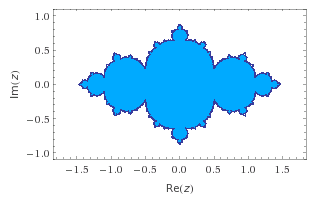
\includegraphics[width=90mm]{img/julia-07001-filled.png}\\
    If $c \neq 0$ then this is non-smooth and a kind of fractal.
\end{frame}

\begin{frame}\frametitle{Background (continued)}
    In 1994 in his book {\it Noncommutative Geometry}, A. Connes introduced a formula for the Hausdorff measure of a Julia set in terms of his quantised calculus:
    \begin{center}
    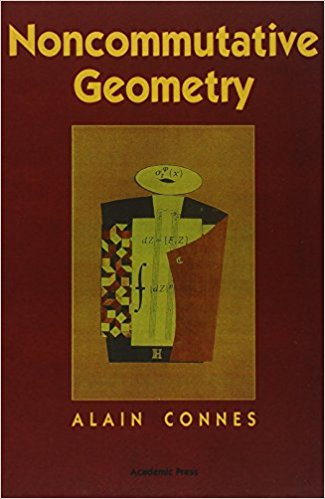
\includegraphics[width=30mm]{img/ncg-book-cover.jpg}
    \end{center}
\end{frame}

\begin{frame}\frametitle{Background (continued)}
    To state the formula properly takes some work, but the key ingredients are as follows: take a Julia set $J$ and let $Z:\Circ\to J$ be the extension
    to the boundary of the conformal equivalence between the exterior of the unit disk and the exterior of $J$:
    \begin{center}
        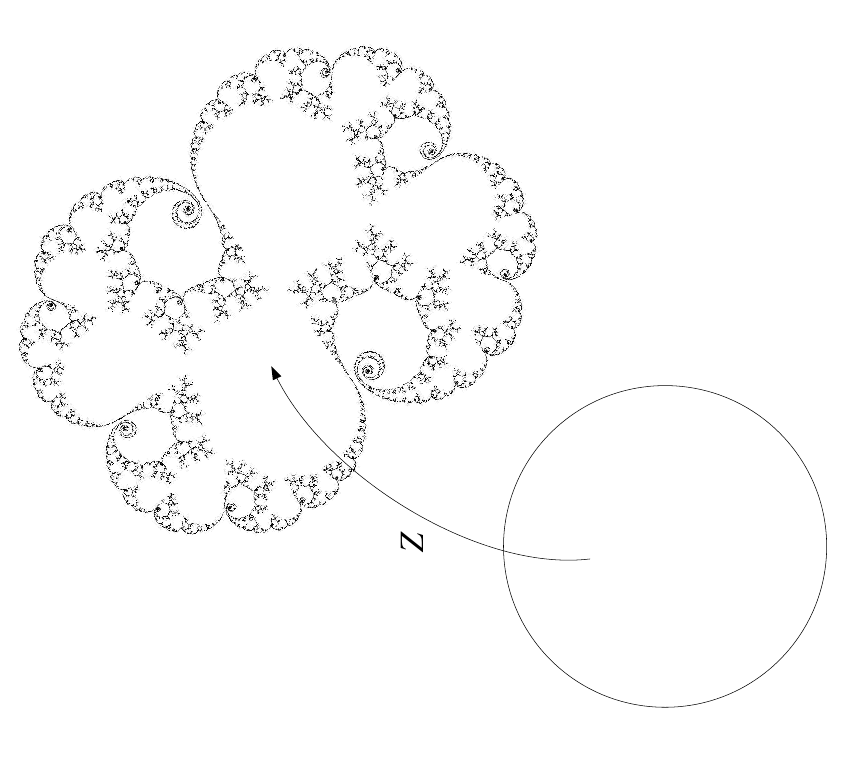
\includegraphics[width=45mm]{img/riemann-mapping.png}
    \end{center}
    $Z$ is typically not differentiable, and it is typically not even of bounded variation.
\end{frame}

\begin{frame}\frametitle{Background (continued)}
    The conformal trace theorem then states that for all continuous normalised traces $\varphi$, there is a constant $C_{\varphi}$ such that:
    \begin{equation*}
        c_{\varphi}\int_J f\,d\lambda_p = \varphi(M_{f\circ Z}|\qd Z|^p).
    \end{equation*}
    where $p$ is the Hausdorff dimension of $J$ and $\lambda_p$ is the $p$-dimensional Hausdorff measure. Connes and Sullivan introduced this formula as a way of computing integrals with respect to the Hausdorff measure on Julia sets.
\end{frame}

\begin{frame}\frametitle{Background (continued)}
    Despite being announced as early as 1994, Connes and Sullivan's proof of the conformal trace theorem was never published.
    
    In our paper we provided a new proof, using operator integration techniques which did not exist in 1994.
\end{frame}

\begin{frame}\frametitle{Background (end)}
    The most technically challenging part of the proof is the so-called ``quantised change of variables formula":
    \begin{equation*}
        |[F,M_{f\circ Z}]|^p-|f'(M_Z)|^p|[F,M_Z]|^p \in \SepPart{1}.
    \end{equation*}
    Where $Z \in C(\Circ)$, and $f$ is a polynomial.
    It is quite easy to show that:
    \begin{equation*}
        [F,M_{f\circ Z}]-f'(M_Z)[F,M_Z] \in \SepPart{p}
    \end{equation*}
    but ``taking a power $p$" is highly nontrivial.
\end{frame}


\section{Part I: Basic conformal dynamics}

\subsection{Julia sets}
% \begin{frame}\frametitle{Context: Dynamical systems}
%     Let $X$ be a set and let $f:X\to X$. Iteration of the function $f$ defines
%     an \emph{iterated function system}. Let $z_0 \in X$, and define
%     \begin{equation*}
%         z_{n+1} = f(z_n),\quad n\geq 0.
%     \end{equation*}
%     %A straightforward description of the asymptotic behaviour of $z_n$
%     Immediate questions which concern us: What is the asymptotic behaviour of $z_n$? How does it depend on $z_0$? There
%     is an enormous literature on this theme.
% \end{frame}

\begin{frame}\frametitle{Complex polynomial dynamics}
    Let $f$ be a polynomial with complex coefficients, and take
    $z_0 \in \Cplx$. consider the recursive sequence:
    \begin{equation*}
        z_{n+1} := f(z_n)\,\quad n\geq 0.
    \end{equation*}
    We are especially interested in studying the asymptotic behaviour of $\{z_n\}_{n\geq 0}$
    for different choices of $z_0 \in \Cplx$. In particular, since $f$ is a polynomial, exactly one of the following happens:
    \begin{enumerate}
        \item{} Either $|z_n| \to\infty$.
        \item{} $\{z_n\}_{n\geq 0}$ remains bounded.
    \end{enumerate}
\end{frame}

\begin{frame}\frametitle{Complex polynomial dynamics}
    The simplest nontrivial example is $f(z) = z^2$. Then $z_k = f^k(z_0) = {z_0}^{2^k}$, and the behaviour
    of $f^{k}(z_0)$ neatly splits into three separate cases:
    \begin{enumerate}
        \item{} If $|z_0| < 1$, then $f^k(z_0)\to 0$ as $k\to\infty$.
        \item{} If $|z_0| = 1$, then $|f^k(z_0)| = 1$ for all $k\geq 0$.
        \item{} If $|z_0| > 1$, then $|f^k(z_0)| \to \infty$ as $k\to\infty$.
    \end{enumerate}
\end{frame}

\begin{frame}\frametitle{Complex polynomial dynamics}
    Pictorially,    
    \begin{center}
    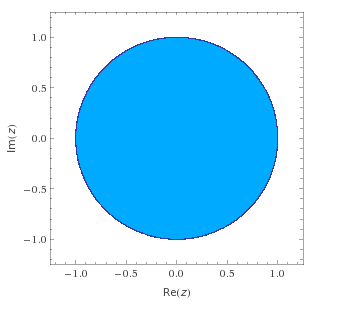
\includegraphics[width=50mm]{img/circle-filled.png}
    \end{center}
    Here, the set of $z_0$ such that $z_n$ remains bounded is coloured in blue. The set of $z_0$ such that $z_n$ is 
    unbounded is white. The boundary of the blue set is highlighted to make it easier to see.
\end{frame}

\begin{frame}\frametitle{Complex polynomial dynamics}
    What if we perturb the polynomial $f(z)=z^2$ slightly? Consider $f(z) = z^2+0.1+0.1i$. 
    
    It is not feasible to determine analytically the behaviour of $\{f^n(z)\}_{n\geq 0}$.
    Instead we use a computer: On a large grid of complex numbers, colour each point $z$
    blue if $f^N(z) < 10$ for some suitably large number $N$.
    
    The result looks like this:
    \begin{center}
        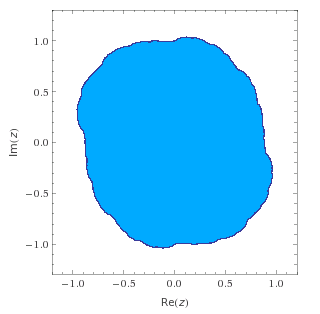
\includegraphics[width=50mm]{img/julia0101-filled.png}
    \end{center}
    Again, the boundary has been highlighted.
\end{frame}

\begin{frame}\frametitle{Complex polynomial dynamics}
    Try $f(z) = z^2+0.1-0.2i$,\\
    \begin{center}
        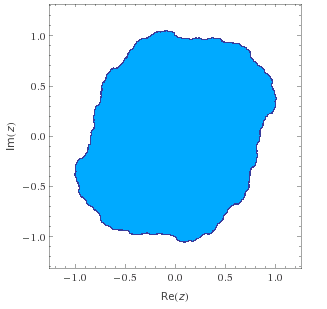
\includegraphics[width=50mm]{img/julia01-02-filled.png}
    \end{center}
\end{frame}

\begin{frame}\frametitle{Complex polynomial dynamics}
    Try $f(z) = z^2+0.2-0.3i$,\\
    \begin{center}
        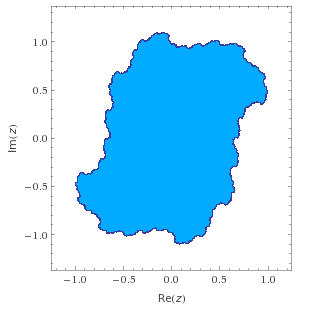
\includegraphics[width=50mm]{img/julia02-03-filled.png}
    \end{center}
\end{frame}

\begin{frame}\frametitle{Complex polynomial dynamics}
    Try $f(z) = z^2+0.3-0.1i$,\\
    \begin{center}
        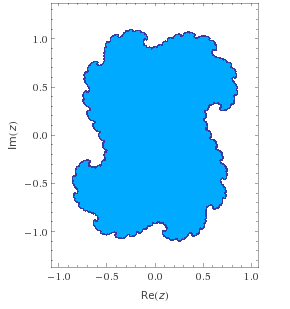
\includegraphics[width=50mm]{img/julia03-01-filled.png}
    \end{center}
\end{frame}

\begin{frame}\frametitle{Complex polynomial dynamics}
    Try $f(z) = z^2-0.7+0.001i$,\\
    \begin{center}
        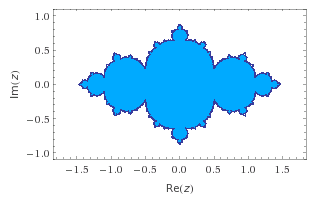
\includegraphics[width=50mm]{img/julia-07001-filled.png}
    \end{center}
\end{frame}

\begin{frame}\frametitle{Complex polynomial dynamics}
    Let try a slightly bigger parameter. Consider $f(z) = z^2+0.5+0.5i$,
    \begin{center}
        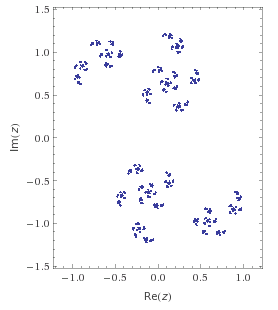
\includegraphics[width=50mm]{img/julia0505.png}
    \end{center}
\end{frame}

\begin{frame}\frametitle{The Mandelbrot set}
    What is going on here?
    Consider the general polynomial:
    \begin{equation*}
        f_c(z) := z^2+c
    \end{equation*}
    with a parameter $c \in \Cplx$.
    Note: any quadratic polynomial can be transformed into some $f_c$ by an affine change of coordinates. 
\end{frame}

\begin{frame}\frametitle{The Mandelbrot set}
    Consider the case $z_0 = 0$ (for simplicity). For which $c$ is $\{f_c^k(0)\}_{k\geq 0}$ bounded?
    Define the Mandelbrot set $M := \{c \in \Cplx\;:\;\{f^k_c(0)\}_{k\geq 0}\text{ is bounded}\}$.
    $M$ can be approximated by a computer:
    \begin{center}
        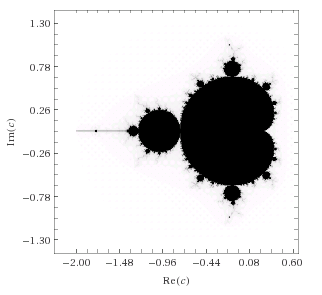
\includegraphics[width=60mm]{img/mandelbrot.png}
    \end{center}
\end{frame}

\begin{frame}\frametitle{The Mandelbrot set}
    A more informative image is this one:
    \begin{center}
        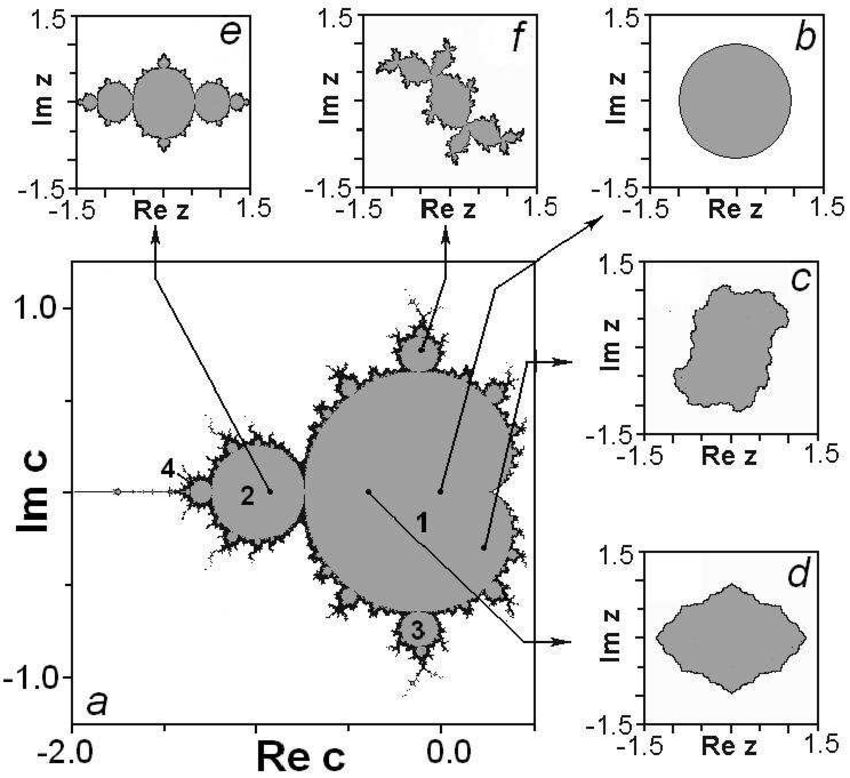
\includegraphics[width=60mm]{img/mandelbrot-with-captions.png}
    \end{center}
\end{frame}

\begin{frame}\frametitle{The Julia set}
    Let $c \in \Cplx$, and consider $f_c(z) = z^2+c$. The \emph{Julia set} of $f_c$ is the boundary
    of the set of points $z \in \Cplx$ such that $\{f_c^n(z)\}_{n\geq 0}$ is bounded.
    \begin{theorem}[Mandelbrot]
        The Julia set $J(f_c)$ is connected if and only if $c \in M$ (the Mandelbrot set).
    \end{theorem}
\end{frame}

\begin{frame}\frametitle{Fixed points}
    The asymptotic behaviour of $\{f^n(z_0)\}_{n\geq 0}$ is best understood by examining the fixed points ($f(z) = z$) of $f$.
    
    A fixed point $\lambda$ is said to be:
    \begin{enumerate}
        \item{} Attracting if $|f'(\lambda)| < 1$,
        \item{} Repelling if $|f'(\lambda)| > 1$,
        \item{} Neutral if $|f'(\lambda)| = 1$.
    \end{enumerate}
    An attracting fixed point $\lambda$ can be called \emph{super-attracting} if $f'(\lambda) = 0$.
\end{frame}

\begin{frame}\frametitle{Fixed points (cont.)}
    The behaviour of $\{f^n(z)\}_{n\geq 0}$ near an attracting fixed point is easily described:
    
    
        If $z$ is sufficiently close to an attracting fixed point $\lambda$, then $f^n(z)\to \lambda$ exponentially fast.
        
        If $\lambda$ is superattracting, then $f^n(z)\to \lambda$ super-exponentially fast.
        
        
    The set of all $z$ such that $f^n(z)\to  \lambda$ as $n\to\infty$ is called the attracting basin of $\lambda$.
    It is easy to see that an attracting basin is open.
\end{frame}

\begin{frame}\frametitle{The main cardioid}
    When does $f(z) = z^2+c$ have an attracting fixed point? 
    
    Let $M_0$ be the set $\{\frac{z}{2}(1-\frac{z}{2})\;:\;|z|<1\}$. $M_0$ is 
    an open subset of the Mandelbrot set $M$ called the \emph{main cardioid}, shown below in red:
    \begin{center}
        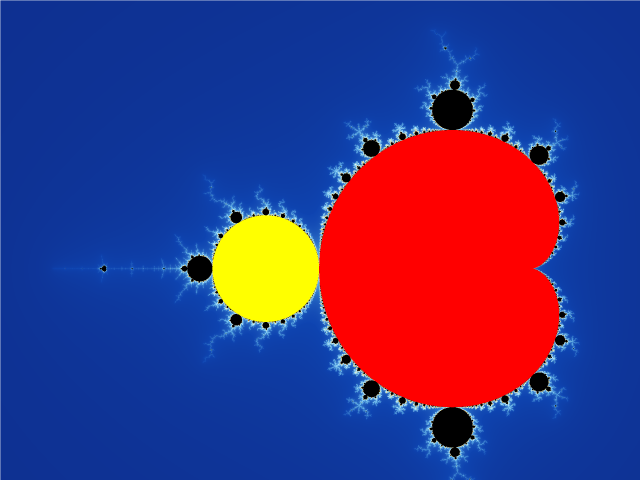
\includegraphics[width=70mm]{img/main-cardioid.png}
    \end{center}
    By definition, if $c \in M_0$ then $f_c$ has an attracting fixed point.
\end{frame}

\begin{frame}\frametitle{The main cardioid}
    The significance of the main cardioid is the following theorem:
    \begin{theorem}
        The Julia set $J(f_c)$ of $f_c$ is a Jordan curve (i.e. homeomorphic to a circle) if and only if $c$ is in the main cardioid $M_0$.
    \end{theorem}
    \begin{proof}[Very rough outline of the proof:]
        The connected components of $\Cplx\setminus J(f_c)$ correspond to the attracting basins of the fixed points of $f_c$. For $c \in M_0$,
        there are exactly two attracting fixed points (one of them at infinity). 
    \end{proof}
\end{frame}

% \begin{frame}\frametitle{Mandelbrot and Julia sets}
%     Let's look at some more pictures:
%     \begin{center}
%         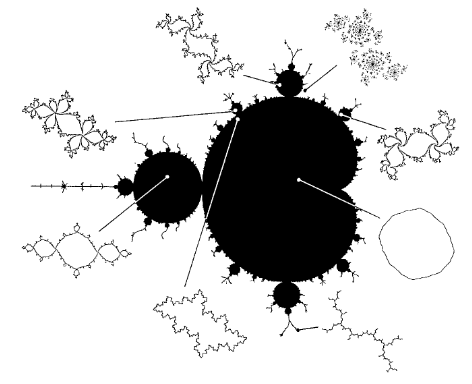
\includegraphics[width=70mm]{img/Falconer-Mandelbrot.png}
%     \end{center}
% \end{frame}

\subsection{Fractal dimensions}
\begin{frame}\frametitle{Hausdorff dimension (reminder)}
    Let $(X,d)$ be a metric space. For $q > 0$, let the $q$-dimensional Hausdorff content of $X$ be:
    \begin{equation*}
        C_q(X) = \inf\{\sum_{j=0}^\infty r_j^q\;:\;X \subseteq \bigcup_{j =0}^\infty B(x_j,r_j)\}.
    \end{equation*}
    
    The Hausdorff dimension of $X$ is defined to be the infimum of the set of $q$ such that $C_q(X) = 0$.
\end{frame}
% 
% \begin{frame}\frametitle{Hausdorff dimension}
%     The Hausdorff dimension is a kind of ``scaling dimension":
%     \begin{center}
%         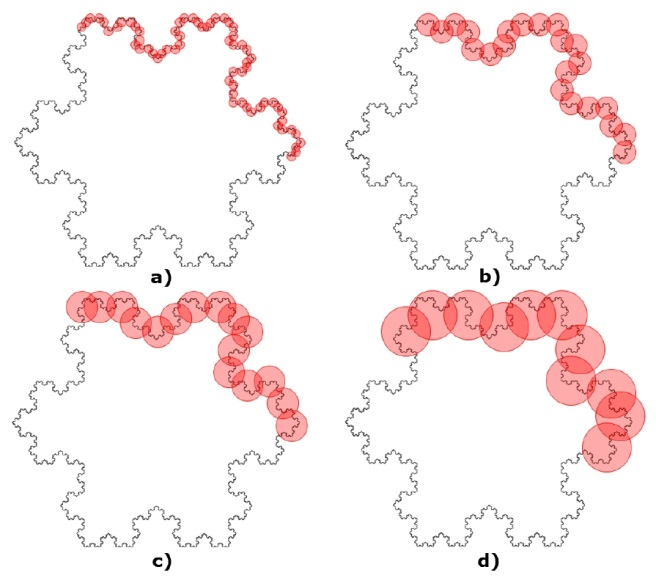
\includegraphics[width=60mm]{img/dimension.jpeg}
%     \end{center}
% \end{frame}

\begin{frame}\frametitle{Hausdorff dimension of Julia sets}
    Fact: If $c$ is in the main cardioid $M_0$ of the Mandelbrot set $M$, then the Julia set $J(f_c)$ is a Jordan curve
    with Hausdorff dimension $p \in [1,2)$. In fact $p = 1$ if and only if $c = 0$.
\end{frame}

\begin{frame}\frametitle{Minkowski content}
    A close relative of Hausdorff dimension is Minkowski dimension.
    Let $X \subseteq \Rl^d$. If $\delta > 0$, let $S_\delta(X) = \bigcup_{x \in X} B(x,\delta)$, or equivalently:
    \begin{equation*}
        S_\delta(X) = \{z \in \Rl^d\;:\;\mathrm{dist}(z,X) < \delta\}.
    \end{equation*}
    
    If there is some $p > 0$ such that:
    \begin{equation*}
        c\delta^{d-p} \leq |S_\delta(X)| \leq C\delta^{d-p}
    \end{equation*}
    for all $\delta > 0$, then $X$ is said to have Minkowski dimension $p$. If $0 < c < C < \infty$, then $X$
    is said to have finite upper and positive lower $p$-dimensional Minkowski content.
\end{frame}

\begin{frame}\frametitle{Conformal dimension}
    Another closely related notion of dimension is conformal dimension (due to Sullivan).
    
    Let $X \subseteq \Cplx$, with $f:X\to X$, and $\nu$ a measure on $X$. The measure $\nu$ is said to be
    $f$-conformal with dimension $p$, if for every open subset $U \subseteq X$ such that $f|U$ is injective, we have:
    \begin{equation*}
        \nu(f(U)) = \int_{U} |f'|^p\,d\nu.
    \end{equation*}
    
    
    


%     Associated to the Hausdorff dimension $p$ there is a $p$-dimensional Hausdorff measure $\lambda_p$. In many cases, 
%     the Hausdorff measure of a ball of radius $r$ scales like $r^p$,
%     \begin{equation*}
%         cr^p \leq \lambda_p(B(z,r)) \leq Cr^p
%     \end{equation*}
%     for some fixed $c,C$ and all $r > 0$.
%     
%     Fact: If $c \in M_0$, and $p$ is the Hausdorff dimension of $J(f_c)$, then the Hausdorff measure $\lambda_p$ on $J(f_c)$
%     is uniquely specified by the above identity. This may not be true for Hausdorff measures in general.
\end{frame}

\begin{frame}\frametitle{Characterising the Hausdorff measure}
    Fact: For Julia sets $J(f_c)$, $c \in M_0$, we have:\\
    Hausdorff dimension $=$ Minkowski dimension\\
    and the Hausdorff measure is the unique $f_c$-conformal measure of dimension equal to $p$, where $p$ is the Hausdorff dimension.
    
    Using the Riesz theorem, we can characterise the Hausdorff measure as follows:
    \begin{theorem}
        The Hausdorff measure $\lambda_p$ of $J(f_c)$ is the unique positive Borel measure such that for all open sets $U\subseteq J(f_c)$ with $f_c|U$ injective,
        and continuous functions $g$ supported in $U$, we have:
        \begin{equation*}
            \int_{f_c(U)} g\,d\lambda_p = \int_U (g\circ f_c)|f_c'|^p\,d\lambda_p.
        \end{equation*}
    \end{theorem}
\end{frame}


\begin{frame}\frametitle{Characterising the Hausdorff measure (cont.)}
    Since $f_c(z) = z^2+c$ we have:
    \begin{equation*}
        f_c^{-1}(f_c(U)) = U\cup -U.
    \end{equation*}
    
    We can moreover say the following:
    \begin{theorem}
        The Hausdorff measure $\lambda_p$ is the unique (up to a constant scalar factor) positive Borel measure such that for all continuous functions $g$ on $J(f_c)$,
        \begin{equation*}
            \int_{J(f_c)} g\,d\lambda_p = \frac{1}{2}\int_{J(f_c)} (g\circ f_c)|f_c'|^p\,d\lambda_p.
        \end{equation*}
    \end{theorem}
    When we prove the conformal trace theorem, we use the above characterisation of the Hausdorff measure.
\end{frame}



\section{Part II: The Conformal trace theorem}

\begin{frame}\frametitle{The main task of the paper}
    Let $g:J(f_c) \to\Cplx$ be a continuous function. In his 1994 book \emph{Noncommutative geometry}, Alain Connes 
    announced a formula for $\int_J g\,d\lambda_p$ given in terms of his ``quantised calculus". We have now completed the proof
    of this formula.
\end{frame}


% \begin{frame}\frametitle{Quantised Calculus: A very rapid introduction}
%     Let $H$ be a (complex, separable) Hilbert space. Let $\mathcal{B}(H)$ denote the algebra
%     of bounded operators on $H$, and let $\|\cdot\|$ denote the operator norm. Given $T \in \mathcal{B}(H)$ and $s \geq 0$, define:
%     \begin{equation*}
%         \mu(s,T) := \inf\{\|T-R\|\;:\;\mathrm{rank}(R) \leq s\}.
%     \end{equation*}
%     The function $s\mapsto \mu(s,T)$ is called the singular value function of $T$.
% \end{frame}
% 
% \begin{frame}\frametitle{Operator $\mathcal{L}_p$ spaces}
%     For $p \in (0,\infty)$, the space $\mathcal{L}_p(H)$ is defined to be the set of operators $T$ such that $\{\mu(n,T)\}_{n\geq 0}$
%     is in $\ell_p$. Similarly, the space $\mathcal{L}_{p,\infty}(H)$ is the set of operators $T$ such that
%     \begin{equation*}
%         \{n^{\frac{1}{p}}\mu(n,T)\}_{n\geq 0}
%     \end{equation*}
%     is bounded. Equivalently, $\{\mu(n,T)\}_{n\geq 0} \in \ell_{p,\infty}$.
%     
%     The spaces $\mathcal{L}_p$ and $\mathcal{L}_{p,\infty}$ are ideals of $\mathcal{B}(H)$ (in the ring-theoretic sense).
% \end{frame}
% 
% \begin{frame}\frametitle{Traces}
%     Let $\mathcal{E}$ be an ideal of $\mathcal{B}(H)$. A functional $\varphi:\mathcal{E}\to \Cplx$ is called a trace if it is invariant under unitary conjugation. That is,
%     for all unitary operators $U$ and $T \in \mathcal{E}$ we have
%     \begin{equation*}
%         \varphi(UTU^*) = \varphi(T).
%     \end{equation*}
%     The most well-known example is the classical trace $\tr$, which can be defined for positive operators $T \geq 0$ by
%     \begin{equation*}
%         \tr(T) = \sum_{n\geq 0} \mu(n,T) = \int_{0}^\infty \mu(s,T)\,ds.
%     \end{equation*}
% \end{frame}
% 
% \begin{frame}\frametitle{Other Traces}
%     There are many more traces on ideals of $\mathcal{B}(H)$.
%     
%     For the ideal $\mathcal{L}_{1,\infty}$:
%     \begin{enumerate}
%         \item{} There exists an uncountable infinity of linearly independent non-trivial traces $\varphi$.
%         \item{} There exist traces $\varphi$ which are continuous in the sense that $|\varphi(T)| \leq C\sup_{n\geq 0} n\mu(n,T)$.
%         \item{} There exist discontinuous traces.
%         \item{} Any continuous trace can be written as a linear combination of positive traces.
%         \item{} All traces vanish on finite rank operators (They are \emph{singular}). 
%     \end{enumerate} 
% \end{frame}

\begin{frame}\frametitle{The Hilbert transform}
    Let $\Circ$ be the unit circle (in the complex plane). The Hilbert space $L_2(\Circ)$ is
    defined with respect to the arc-length measure (the Haar measure).
    
    There is the trigonometric orthonormal basis for $L_2(\Circ)$,
    \begin{equation*}
        e_n(z) = z^n,\quad n\in \Itgr, z \in \Circ.
    \end{equation*}
    The Hilbert trasform $F$ is defined on the basis $e_n$ by $Fe_n = \sgn(n)e_n$.
\end{frame}

\begin{frame}\frametitle{Quantised differentials}
    If $f$ is a bounded function on $\Circ$, then pointwise multiplication
    by $f$ defines a bounded linear operator $M_f$ on $L_2(\Circ)$. 
    Connes calls the commutator $i[F,M_f]$ the ``quantised differential" of $f$.
    
    The name is intended to imply that this is something like a differential $df$. So we use the symbol $\qd f$,
    \begin{equation*}
        \qd f := i[F,M_f].
    \end{equation*}
\end{frame}

\begin{frame}\frametitle{B\"ottcher coordinates}
    
    The following is due to L. B\"ottcher:
    \begin{theorem}
        Let $f$ be a polynomial of degree $d \geq 2$. There exists a conformal map $Z$:
        \begin{equation*}
            Z:\{|z| > 1\}\to \text{Attracting basin of }\infty.
        \end{equation*}
        such that $f(Z(z)) = Z(z^d)$, for all $|z| > 1$.
    \end{theorem}
    If $J(f_c)$ is a Jordan curve, then Carath\'eodory's theorem implies that $Z$ has continuous extension:
    \begin{equation*}
        Z:\Circ\to J(f_c)
    \end{equation*}
    such that $Z(z^2) = f_c(Z(z))$ for all $z \in \Circ$.
%       Let $c \in M_0$ (the main cardioid of the mandlebrot set), and let $c \neq 0$ so that $J(f_c)$ is a Jordan curve with Hausdorff dimension $1 < p < 2$. Since $J$ is a Jordan curve,
%       there is a conformal mapping $Z$ from the exterior of the unit disc to the exterior of $J(f_c)$,
%       \begin{center}
%           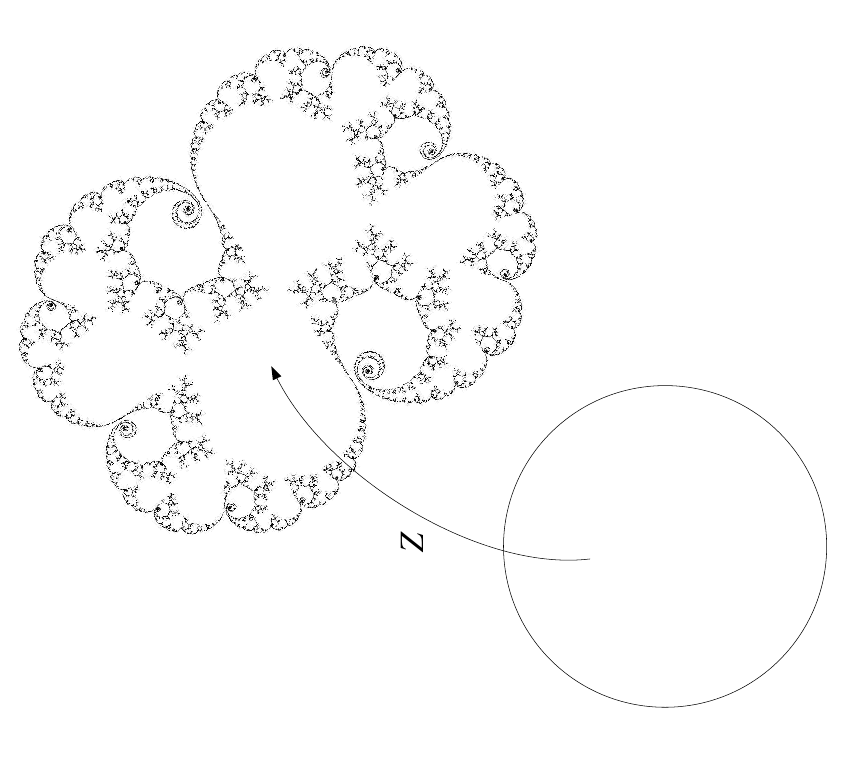
\includegraphics[width=60mm]{img/riemann-mapping.png}
%       \end{center}
%       There is a theorem of complex analysis (Carath\`eodory's theorem) which implies that $Z$ extends to a continuous function on the unit circle $\Circ := \{z \in \Cplx\;:\;|z|=1\}$
%       to $J(f_c)$. We can choose $Z$ so that it satisfies the functional equation
%       \begin{equation*}
%         Z(z)^2+c = Z(z^2),\quad z \in \Circ.
%       \end{equation*}
\end{frame}

\begin{frame}\frametitle{Description of the Conformal Trace Formula}
     Let $f$ be a continuous function on the Julia set $J(f_c)$. Then the operator
     \begin{equation*}
        M_{f\circ Z}|\qd Z|^p = M_{f\circ Z}|[F,M_Z]|^p
     \end{equation*}
     is some kind of ``$p$-dimensional density" on the Julia set $J(f_c)$ (in the language of quantised calculus).
     
     Motivated by noncommutative geometry, one might guess that the correct way of ``integrating" this density is to take a trace.
\end{frame}

\begin{frame}\frametitle{Description of the Conformal Trace Formula}
    \begin{lemma}
        The quantised differential $\qd Z$ (i.e., the commutator $[F,M_Z]$) is in the ideal $\Lc_{p,\infty}$.
    \end{lemma}
    Hence, the operator $M_{f\circ Z}|\qd Z|^p$ is in $\Lc_{1,\infty}$.
\end{frame}

\begin{frame}\frametitle{Description of the Conformal Trace Formula}
    \begin{theorem}
        Let $\varphi$ be a continous trace on $\Lc_{1,\infty}$. Then there is a constant $K(\varphi,c)$ such
        that for all $f \in C(J(f_c))$,
        \begin{equation*}
            \varphi(M_{f\circ Z}|\qd Z|^p) = K(\varphi,c)\int_{J(f_c)} f\,d\lambda_p
        \end{equation*}
        where $\lambda_p$ is the $p$-dimensional Hausdorff measure on $J(f_c)$.
        Also, there exist traces $\varphi$ such that $K(\varphi,c) > 0$.
    \end{theorem}
\end{frame}

\begin{frame}\frametitle{Equivalent statement of the Conformal trace theorem}
    Recall that the Hausdorff measure can be characterised as the unique $f_c$-conformal measure of dimension $p$. 
    
    Let $\ell_{\varphi}$ be the linear functional:
    \begin{equation*}
        \ell_{\varphi}(g) = \varphi(M_{g\circ Z}|\qd Z|^p).
    \end{equation*}
    By the Riesz theorem, there is some measure $\nu$ such that $\ell_\varphi$ is integration against $\nu$.
    It therefore suffices to show the following:
    \begin{enumerate}
        \item{} For all continuous $g:J(f_c)\to \Cplx$, we have:
            \begin{equation*}
                \ell_{\varphi}(g) = \frac{1}{2}\ell_\varphi((g\circ f_c)|f_c'|^p).
            \end{equation*}
        \item{} $\ell_{\varphi} > 0$, for at least some $\varphi$.
    \end{enumerate}
\end{frame}

\subsection{Non-trivality}

\begin{frame}\frametitle{Non-triviality (cont.)}
    First, we can show the ``non-triviality" component.
    \begin{theorem}
        Let $\mathcal{C}$ be a Jordan curve with finite upper and positive lower $p$-Minkowski content, and let $\zeta:\Circ\to \mathcal{C}$ be the continuous extension of a conformal equivalence of the open unit disk
        and the interior of $\mathcal{C}$. Then $\qd \zeta \in \Lc_{p,\infty}$, and for all dilation invariant extended limits $\omega$ such that $\omega\circ \log$ is still dilation invariant, we have:
        \begin{equation*}
            \tr_\omega(|\qd \zeta|^p) > 0.
        \end{equation*}
    \end{theorem}
\end{frame}

\begin{frame}\frametitle{Non-triviality (cont.)}
    Idea of the proof:    
    If $\omega$ satisfies the stated conditions, then:
    \begin{equation*}
        \tr_\omega(|\qd \zeta|^p) = (\omega\circ \log)\left(t\mapsto \frac{1}{t}\tr(|\qd \zeta|^{p(1+1/t)})\right)
    \end{equation*}
    So it suffices to show that:
    \begin{equation*}
        \liminf_{s\to 0} s\cdot \tr(|\qd \zeta|^{p+s}) > 0.
    \end{equation*}
%     Which can be achieved with the integral formula:

\end{frame}

\begin{frame}\frametitle{Non-triviality (cont.)}
    A theorem of Peller gives us the equivalence:
    \begin{equation*}
        \tr(|\qd \zeta|^{p+s}) \approx \int_{\mathbb{D}} |\zeta'(z)|^{p+s}(1-|z|^2)^{p+s-2}\,dzd\overline{z}.
    \end{equation*}
    According to the Koebe $1/4$-theorem,
    \begin{equation*}
        \dist(\zeta(0),\mathcal{C}) \leq |\zeta'(0)| \leq 4\dist(\zeta(0),\mathcal{C})
    \end{equation*}
    A change of coordinates yields:
    \begin{equation*}
        \frac{1}{4}(1-|z|^2)|\zeta'(z)| \leq \dist(\zeta(z),\mathcal{C}) \leq (1-|z|^2)|\zeta'(z)|
    \end{equation*}
    for all $z \in \Disc$.    
\end{frame}

\begin{frame}\frametitle{Non-triviality (cont.)}
    In summary:
     \begin{equation*}
         \tr(|\qd \xi|^{p+s}) \approx \int_{\mathrm{int}\mathcal{C}} \mathrm{dist}(z,\mathcal{C})^{p+s-2}\,dzd\overline{z}.
     \end{equation*}
    The question is now reduced to a purely geometric problem concerning $\mathcal{C}$.
\end{frame}

\begin{frame}\frametitle{Non-triviality (cont.)}
    Split up $\mathrm{int}\mathcal{C}$ into regions:
    \begin{equation*}
        A_k = \{z \in \mathrm{int}\mathcal{C}\;:\; \dist(z,\mathcal{C}) \in [\lambda^{-k-1},\lambda^{-k})\}.
    \end{equation*}
    Then,
    \begin{equation*}
        \int_{\mathrm{int}\mathcal{C}} \mathrm{dist}(z,\mathcal{C})^{p+s-2} \,dzd\overline{z} \geq \sum_{k\geq 0} \lambda^{-k(p+s-2)}|A_k|.
    \end{equation*}
    with $|A_k| = |S_{\lambda^{1-k}}(\mathcal{C})\cap \mathrm{int}(\mathcal{C})|-|S_{\lambda^{-k}}(\mathcal{C})\cap \mathrm{int}(\mathcal{C})| \geq B\lambda^{-k(2-p)}$
    for sufficiently big $\lambda$.
    
    This gives,
    \begin{equation*}
        \liminf_{s\to 0} s\cdot \tr(|\qd \zeta|^{p+s}) > 0.
    \end{equation*}
\end{frame}


\subsection{Proving conformality}
\begin{frame}\frametitle{Proving conformality}
    The remaining task is to show that:
    \begin{equation*}
        \ell_{\varphi}(g) = \frac{1}{2}\ell_{\varphi}((g\circ f_c)|f_c'|^p).
    \end{equation*}

    Recall that we have the B\"ottcher equation:
    \begin{equation*}
        Z(z^2) = f_c(Z(z)).
    \end{equation*} 
    Let $U$ be the partial isometry on $L_2(\Circ)$ given by $U(z^n) = z^{2n}$. Then,
    \begin{equation*}
        UM_ZU^* = M_{f_c\circ Z}.
    \end{equation*}
    we also have $U^*U = 1$ and $UU^* = P$ is the projection $P(z^n) = z^n$ if $n$ is even and $0$ if $n$ is odd.
    
    It is important that $U$ commutes with the Hilbert transform $F$.
\end{frame}

\begin{frame}\frametitle{Proving conformality (cont.)}
    Then,
    \begin{align*}
        \varphi(M_{g\circ Z}|\qd Z|^p) &= \varphi(U^*UM_{g\circ Z}|\qd Z|^p)\\
                                       &= \varphi(M_{g\circ f_c\circ Z}U|[F,M_{Z}]|^pU^*)\\
                                       &= \varphi(M_{g\circ Z}|[F,M_{f_c\circ Z}]|^pUU^*)\\
                                       &= \varphi(M_{g\circ f_c\circ Z}|\qd (f_c\circ Z)|^pP).
    \end{align*}
    A further argument using unitary invariance shows that:
    \begin{align*}
        \varphi(M_{g\circ f_c\circ Z}|\qd (f_c\circ Z)|^pP) = \frac{1}{2}\varphi(M_{g\circ f_c\circ Z}|\qd (f_c\circ Z)|^p)
    \end{align*}
\end{frame}


\begin{frame}\label{The quantised chain rule}
    The following is called by Connes a ``quantised chain rule". Let $f$ be a polynomial. Then:
    \begin{equation*}
        |\qd (f\circ Z)|^p-|f'(M_Z)|^p|\qd Z|^p \in \SepPart{1}.
    \end{equation*}
    Proving the above identity is the most technically challenging part of the proof, requiring the operator integration tricks developed in the preceding talk.
\end{frame}

\begin{frame}\frametitle{The quantised chain rule (cont.)}
    We have,
    \begin{equation*}
        [M_f,[F,M_Z]] = [[M_f,F],M_Z]
    \end{equation*}
    Since $f$ is a polynomial, the commutator $[M_f,F]$ is finite rank.
    
    Thus, we have:
    \begin{equation*}
        M_{z^n}[F,M_Z]M_{z^{-n}}-[F,M_Z] \in \SepPart{p}. 
    \end{equation*}
    This (highly nontrivally) implies that:
    \begin{equation*}
         |M_{z^n}[F,M_Z]M_{z^{-n}}|^p-|[F,M_Z]|^p \in \SepPart{1}.
    \end{equation*}
    Since $M_{z^n}$ is unitary, we get:
    \begin{equation*}
        [M_{z^n},|[F,M_Z]|^p] \in \SepPart{1}.
    \end{equation*}
\end{frame}

\begin{frame}\frametitle{The quantised chain rule (cont.)}
    Hence for all polynomials $f$,
    \begin{equation*}
        [M_f,|\qd Z|^p] \in \SepPart{1}.
    \end{equation*}
    An approximation argument allows us to state the above for all continuous $f$ as well.
    
    Fact: we also have $[M_f,|\qd Z|] \in \SepPart{p}$.
    
    Since $[M_{Z}^n,[F,M_Z]] \in \SepPart{p}$, we have that:
    \begin{equation*}
        [F,M_{Z}^n] \in nM_Z^{n-1}[F,M_Z]+\SepPart{p}.
    \end{equation*}
\end{frame}

\begin{frame}\frametitle{The quantised chain rule (cont.)}
    By linearity,
    \begin{equation*}
        [F,f(M_Z)] - f'(M_Z)[F,M_Z] \in \SepPart{p}.
    \end{equation*}
    So,
    \begin{equation*}
        |[F,f(M_Z)]|^p - |f'(M_Z)[F,M_Z]|^p \in \SepPart{1}.
    \end{equation*}
    Using the identity $|AB| = ||A|B|$, and $[M_{|f'\circ Z|^{1/2}},|[F,M_Z]|] \in \SepPart{p}$ we have
    \begin{equation*}
        |\qd f\circ Z|^p - (|f'(M_Z)|^{1/2}|\qd Z||f'(M_Z)|^{1/2})^p \in \SepPart{1}.
    \end{equation*}
\end{frame}

\begin{frame}\frametitle{The quantised chain rule (cont.)}
    Using the advanced operator integration techniques from the preceding talk:
    \begin{equation*}
        |f'(M_Z)|^p|\qd Z|^p- (|f'(M_Z)|^{1/2}|\qd Z||f'(M_Z)|^{1/2})^p \in \SepPart{1}.
    \end{equation*}
    This finally gives us the quantised chain rule:
    \begin{equation*}
        |\qd (f\circ Z)|^p - |f'(M_Z)|^p|\qd Z|^p \in \SepPart{1}.
    \end{equation*}
\end{frame}

\begin{frame}\label{The end of the proof}
    The quantised chain rule gives us:
    \begin{equation*}
        \varphi(M_{g\circ f_c\circ Z}|\qd (f_c\circ Z)|^p) = \varphi(M_{g\circ f_c\circ Z}|f_c'(M_Z)|^p|\qd Z|^p).
    \end{equation*}
    Which is exactly what we needed.
\end{frame}

\subsection{Further directions}
\begin{frame}\frametitle{Further directions}
    \begin{itemize}
        \item{} What is the dependence of $K(\varphi,c)$ on $\varphi$?
        \item{} Can a similar result be stated for Julia set of more general polynomials (or even non-polynomials)?
        \item{} Can we provide a similar result for Hausdorff measures on other Jordan curves in the plane? (such as a Koch snowflake)
    \end{itemize}
    At present, very little is known.
\end{frame}

\subsection{The end.}
\begin{frame}
    Thank you for listening!
%     
%     More information on operator ideals and their traces can be found in:\\
%     Lord, Steven; Sukochev, Fedor; Zanin, Dmitriy {\bf Singular traces}. Theory and applications. De Gruyter Studies in Mathematics, 46. {\emph De Gruyter, Berlin}, 2013.\\
%     
    Further reading:\\
    Good references for Julia sets and conformal dynamics are,\\
    Carleson and Gamelin, \emph{ Complex Dynamics}, 1993\\
    Milnor, \emph{Dynamics in One Complex variable}, 2006.\\
    
    More information on the quantised calculus may be found in:\\
    Connes, \emph{Noncommutative geometry}, 1994.
\end{frame}

% \begin{frame}\frametitle{Description of the conformal trace formula}

% \end{frame}
% 
% \begin{frame}\frametitle{Description of the conformal trace formula}
%     The space $L_2(\Circ)$ of square integrable functions on $\Circ$ (with respect to the arc length measure) has a basis $\{e_n\}_{n\in \Itgr}$ given by $e_n(z) = z^n$. The Hilbert transform $F$
%     is the linear map defined on $e_n$ by $Fe_n = \sgn(n)e_n$.
% \end{frame}

\end{document}
